\documentclass[abstract=on,9pt,twocolumn]{scrartcl}

\usepackage{ucs}
\usepackage[utf8x]{inputenc}
\usepackage[T1]{fontenc}
\usepackage[english]{babel}

%\usepackage{graphics}%	images other than eps

\usepackage[paper=a4paper,top=2cm,left=1.5cm,right=1.5cm,bottom=2cm,foot=1cm]{geometry}

\usepackage{relsize}%	relative font sizes

\usepackage[retainorgcmds]{IEEEtrantools}%	IEEEeqnarray
\setlength{\IEEEnormaljot}{4\IEEEnormaljot}

\usepackage{graphicx}
\usepackage{epstopdf}
\usepackage{indentfirst}
\usepackage{hyperref}
\usepackage{cleveref}
%\usepackage[noabbrev]{cleveref}
\usepackage{listings}
\usepackage{color}
\usepackage{todonotes}

%%%%%%%%%%%%%%%%
%  title page  %
%%%%%%%%%%%%%%%%
\titlehead{University of Minho \hfill Master's Degree in Informatics Engineering\\	Department of Informatics \hfill Computer Graphics}

\title{JSARToolKit}

\subtitle{Augmented Reality applied to a Pokémon\textregistered\ Game}

\author{Ana Catarina Macedo\\\texttt{\smaller axxxx@alunos.uminho.pt}
\and Miguel Palhas\\\texttt{\smaller pg19808@alunos.uminho.pt}
\and Pedro Costa\\\texttt{\smaller pg19830@alunos.uminho.pt}}

\date{Braga, June 2012}

\subject{Virtual and Augmented Reality}


%%%%%%%%%%%
%  Hacks  %
%%%%%%%%%%%

%	Paragraph (title) with linebreak
\newcommand{\paragraphh}[1]{\paragraph{#1\hfill}\hfill

}

%	Add "Appendix" to the appendices titles, but not to the references
\usepackage{ifthen}
\newcommand*{\appendixmore}{%
  \renewcommand*{\othersectionlevelsformat}[1]{%
    \ifthenelse{\equal{##1}{section}}{\appendixname~}{}%
    \csname the##1\endcsname\autodot\enskip}
  \renewcommand*{\sectionmarkformat}{%
    \appendixname~\thesection\autodot\enskip}
}




\begin{document}
\maketitle

\begin{abstract}
This document describes the implementation of a game based on the classic Pokémon\textsuperscript{\textregistered} using the JSARToolKit to allow player interactivity using Augmented Reality. Despite the lack of resources, the JSARToolKit was used to build a basic sample which allowed to place virtual elements together with a real-time image. The game was implemented using the markers as place for the monsters to appear allowing interaction by changing the marker visibility. Several features of the original game were replicated, such as the capture system, the evolution and the Pokédex.
\end{abstract}
\section{Introduction}
\label{sec:intro}

ARToolKit is a library implemented in C/C++ for building Augmented Reality (AR) applications. Due to the abstraction and mechanisms it provides, several ports of this library have been made to other languages, extending its functionalities to other programmers. The nyARToolKit was a direct port of the original library to the Java language. From this, the FLARToolKit library was born, which ported the functionalities to ActionScript (Flash). This last port was then used by Ilmari Heikkinen to create the library behind this project: the JSARToolKit, a port of the FLARToolKit library to build AR applications in Javascript.

This document describes the implementation of an interactive application which follows a mechanic analogous to that of the role-playing game Pokémon\textregistered, using the JSARToolKit library to implement the interactive component using Augmented Reality. This application revolves the original game's premise where the goal is to collect all the different Pokémons, but the concept is simplified: the goal is to capture the monsters which show up randomly in the markers by interfering with their recognition. The game mechanics is essentially meant for continuous playing or goal oriented around a scoring system limited by time.

\Cref{sec:jsartoolkit} describes how the JSARToolKit library was used to identify the markers in the player webcam stream and how WebGL was used to add virtual elements to the scene. In \cref{sec:game}, the game mechanics, how the markers are managed and the scoring system are explained. The conclusion is presented in \cref{sec:conclusion}. Additionally, a description of the setup required to test the game is presented in \cref{sec:setup}.

\section{JSARToolKit}
\label{sec:jsartoolkit}

The application of the JSARToolKit library to this project is present in the implementation of a functionality similar to that of the basic sample in the original ARToolKit library. In that sample, the library is used to recognize the markers in the webcam's video stream, and to retrieve the transformation matrices which are used to place 3D models in the same ``place'' (position, orientation and scale). The JSARToolKit library does possess a similar sample in its release bundle, but the code not reusable due to lack of structure and documentation and the use of specific auxiliary libraries (with little or no documentation at all) and deprecated code. Other specific tutorials exist among the online community, but these suffer from the same problems of lack of documentation and/or outdated code which is no longer functional.

The first step in this project was setting the system to allow the browser to use the webcam stream in real time. Such preparation is explained in \cref{sec:setup}. The webcam stream is loaded to a \texttt{video} html tag, and in each frame a canvas is redrawn using the stream (the image in this canvas is later analyzed in the search for markers). The second step involved recreating the basic sample by adding the marker recognition to the result of the first step through the analysis of the code in the mentioned faulty tutorials and samples.

\todo[inline]{Add here a camera.html screenshot}

The JSARToolKit library uses a raster object which receives a canvas holding the images to analyze. This raster is then used by a detector which retrieves the information about all the markers present in the scene\footnote{The library is quite sensible to light variations and color changes. It is possible for a marker to be present in the image while the detector can not identify it (weaker ilumination, shadow).}. In each frame, the detector is used in the image retrieved from the webcam and each marker is properly identified and added to a structure.

The lack of stability in the detector (it is common for markers to disappear every other frame) is compensated by using an aging process for each marker. In each frame, the marker's age is incremented. Everytime the detector finds a given marker, its age is reset to zero. When the marker's age reaches a given threshold, it is deleted from the structure.

The second part of the basic sample places a cube on the marker. For this, the Three.js library was used, which allowed to remove much of the complexity intrinsic to the creation of a virtual scene using WebGL.

\todo[inline]{Add here a basic.html screenshot}
\Section{GAME}
\label{sec:game}

The Pokémon\textsuperscript{\textregistered} game, released for the Nintendo\textsuperscript{\textregistered} Game Boy\textsuperscript{\textregistered} in 1996 in two complementary versions, is a role-playing game based on the premise of a young man who takes the goal of finding and capturing each one of the 150 Pokémons (\textit{pocket monsters}).

The various Pokémons were attainable in different ways (some only existed in one of the versions and had to be traded), the most common being the ``tall grass'' -- one of the many visual elements to represent an area where a Pokémon could appear. Other Pokémons could only be obtained by evolving a previous form to a certain level.

The act of catching a wild Pokémon consisted in weakening it through battle (although this was often unnecessary) and using an item called PokéBall. If the Pokémon settled inside the ball, it would be considered caught. If it broke free, the battle would continue, giving the player a chance to retry. Some Pokémon were also able to flee from a battle.

The implemented game follows the same premiss but uses a mechanic different than that of the original game, thus including an interactive component with augmented reality. In this game, the markers represent the places where Pokémons can appear (``tall grass''). While a marker is visible, it is possible for a Pokémon to appear in it. If such happens, the player may hide the marker (equivalent to throwing a PokéBall). Due to the already described process of aging the markers, it takes a few frames for the action of the player to be recognized, after which the image of the Pokémon in the hidden marker changes into that of a PokéBall. Each Pokémon holds a different catch rate, and depending on the value generated in each frame, the Pokémon may settle (consequently being accepted as caught), may break free or may just shake the PokéBall. If the Pokémon is caught, the PokéBall simply disappears, and the process starts over. If the Pokémon breaks free, the player must reveal the marker and conceal it again. If the PokéBall shakes, the decision process is repeated in the next frame. A Pokémon is allowed to flee after some frames while idle or after breaking free.

\begin{figure}
	\begin{center}
		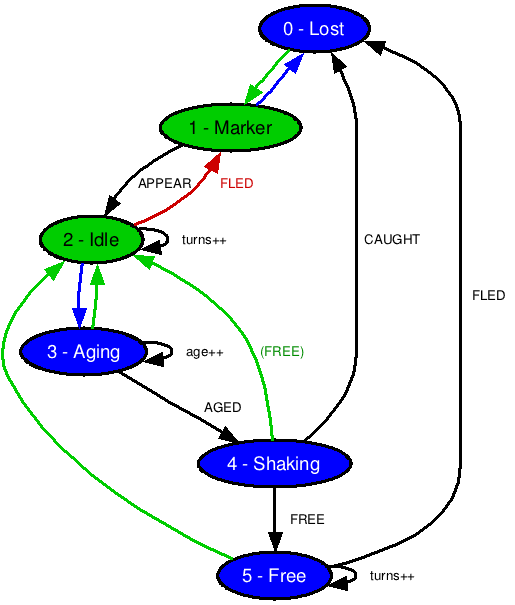
\includegraphics[width=\columnwidth]{report/images/marker.png}
	\end{center}
	\caption[Marker States]{Finite State Machine which describes the markers during the game. States in blue represent an invisible marker, states in green represent a visible one. Green and blue arrows represent a change in the marker visibility. Black and red arrows represent conditional events.}
	\label{fig:fnm}
\end{figure}

Each marker is represented in the game as a Finite State Machine, described in \Cref{fig:fnm}. The implemented states are as follows:
\begin{description}
	\item[Lost (hidden)]{Every marker starts in this state and changes only when revealed.}
	\item[Marker (revealed)]{Empty marker. If hidden, the state changes back to Lost. In each frame, a Pokémon is selected and $\xi\in\left[0,1\right]$ is generated. If $\xi$ is less than the probability for that Pokémon to appear, the Pokémon is assigned to the marker and the state changes to Idle. Otherwise it remains in the same state.}
	\item[Idle (revealed)]{The Pokémon is kept on the marker, waiting for player interaction. If the marker is hidden, the state changes to Aging. After some frames (turns) without interaction, in each frame $\xi\in\left[0,1\right]$ is generated and if $\xi$ is less than the probability for the Pokémon to flee, the Pokémon is removed from the marker and the state changes back to Marker. Otherwise it remains in the same state.}
	\item[Aging (hidden)]{As described, this state sole purpose is to compensate the lack of stability in the marker detection mechanism. Each frame the age of the marker is incremented. When the age reaches the configured threshold, the state changes to Shaking. If the marker is revealed, the state changes back to Idle.}
	\item[Shaking (hidden)]{In each frame, $\xi\in\left[0,1\right]$ is generated. If below the catch rate $c$ of the Pokémon, it is considered caught and the marker information is deleted (thus changing the state to Lost). If above $1-c$, the state is changed to Free. Otherwise, the process is repeated in the next iteration. If the marker is revealed, the Pokémon breaks free and the state is changed back to Idle.}
	\item[Free (hidden)]{If the marker is revealed, the state changes to Idle. After some frames without interaction, $\xi\in\left[0,1\right]$ is generated and if $\xi$ is below the probability of the Pokémon fleeing, the marker is deleted (thus changing the state to Lost).}
\end{description}

\begin{figure}
	\begin{center}
		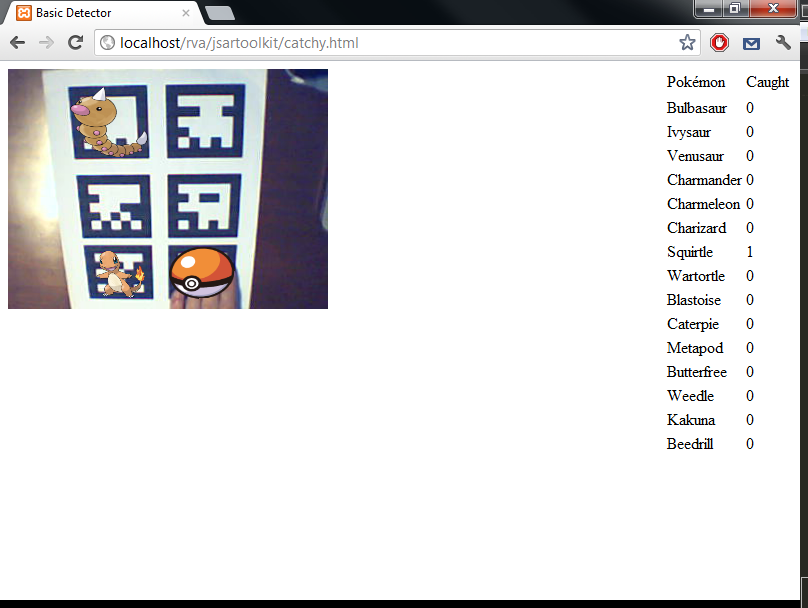
\includegraphics[width=\columnwidth]{report/images/catchy.png}
	\end{center}
	\caption[Game]{The canvas can be seen which includes the camera video feed, as well as some Pokémons appearing on randomly chosen markers. The bottom right marker is currently being obstructed by the user's hand, so a pokéball is shown instead, meaning the player is currently capturing that pokémon.}
	\label{fig:catchy}
\end{figure}

\SubSection{EVOLUTION}
\label{sec:evolution}

In order to simulate the process of evolution, the concept of level is simplified to that of how many times a form as been caught. The subsequent forms are then locked with the required number of times the previous form needs to be caught in order to unlock it. The act of unlocking is automatic: when a Pokémon is selected in the Marker state, if the number of times the previous form has been caught is greater than the lock value, the Pokémon is accepted.

As an example, assume three forms $X$, $Y$ and $Z$ where $Y$ is the evolution of $X$ and $Z$ is the evolution of $Y$. Also, assume $C_{F}$ and $L_{F}$ to be the number of times the form $F$ has been caught and the lock value of the form $F$, respectively. Since $X$ is the base form, $L_{X}=0$. If $L_{Y}=y$, it means that the form $Y$ will not appear while $C_{X}<y$. Similarly, if $L_{Z}=z$, the form $Z$ will not appear while $C_{Y}<z$.
\SubSection{POKÉDEX}
\label{sec:pokedex}

In the original game, the player is able to keep track of the Pokémons he/she has caught using the Pokédex, a fictional device which records the informations about all the seen and caught Pokémons in a numbered list.

Since a similar logic feature was required to implement the evolution system, a \texttt{table} tag was added to the page of the game with the scoreboard of each Pokémon. This table is automatically updated using the Document Object Model\footnote{(DOM) Convention used to access the elements of an HTML page using an object-oriented paradigm, regarding the scripting language used.} methods.

\Section{CONCLUSION}
\label{sec:conclusion}

In this document the implementation of a game based on the classic for portable devices Pokémon\textsuperscript{\textregistered} was described along with the JSARToolKit library which provided the abstraction necessary for Augmented Reality to be used as the interaction method.

The implemented application used the WebRTC standard with an experimental release of Google Chrome to access the player webcam stream in real-time. The stream is then used in the JSARToolKit library to detect the markers and retrieve the information necessary to place the Pokémons on top of them.

The game mechanics was implemented using a robust Finite State Machine model which predicts the changes in the marker visibility, the interaction of the player and the mechanisms required for the game logic (such as the Pokémon appearing, being caught or fleeing).

Additional features, such as the Pokédex or an analogy to the evolution was added to improve the quality of the game.

The JSARToolKit library proved to be the hardest challenge in this project, mainly due to the lack of documentation, both in and out of the source code. Aside from the source code itself, which due to the unfamiliarity with the Javascript language was not viable to analyze completely, only two resources online were found, both written by the author of the library. Yet, both those resources were filled with non functional, deprecated and very specific code. Understanding the library, as well as all the other elements required to make it work represented the most challenging part of the project. Shamefully, this lack of documentation seems to be a common practice in the Computer Graphics community.

Although perfectly functional, and complete under the proposed goals for this project, much can be done to improve this game. Aside from the obvious design improvements, features like the different types of evolutions and floating text replacing the console would improve greatly the player experience. On a more general note, the concept of battle was ignored so far, but it may be possible to incorporate an analog feature in this game.

\bibliographystyle{IEEE}
\bibliography{references}

\appendix

\section{Setup}
\label{sec:setup}

The webcam stream is an essencial part of this project. Yet, obtaining this stream in a web browser is still an experimental feature, not widely available. This project was particularly tested and designed for the \textit{Google Chrome}\footnote{\url{http://chrome.google.com}}. The standard used in this project was designed (and at the date of this document it is still in development) by the WebRTC (Real-time Communications) initiative\footnote{\url{http://www.webrtc.org/home}}. At the date, to obtain a WebRTC enabled binary of Google Chrome, a canary build must be obtained (links in the WebRTC website).

To test this project, it is required that the \texttt{MediaStream} flag is activated in the browser. This can be done temporarily by calling the Google Chrome (RTC) executable with the argument \texttt{--enable-media-stream}, or permanently by acessing the address \url{chrome://flags} and enabling the flag in that page (the process can be reverted in the same page). After this, when acessing the game page, a bar will appear below the Favorites, asking if the user allows the browser to use the webcam. Allowing will start the game.
%\input{report/92_source}

\end{document}
